\documentclass[english,11pt,twoside,a4paper]{article}
\usepackage[left=2cm,top=1cm,right=2cm,nohead,nofoot]{geometry}
\usepackage[utf8]{inputenc}
\usepackage{hyperref}
\usepackage{amssymb}
\usepackage{graphicx}
\begin{document}
\author{
  Niemistö, Jesse
  \and
  Muona, Leo
  \and
  Hilden, Matias
}
\title{Requirements and design}

\maketitle

\section{Introduction}
This document includes requirements, features and design of our turret for Intelligent Embedded Systems -course (University of Helsinki course number 582711). For our project we chose to create an "intelligent" turret inspired by video game Portal by Valve Company. This document describes the intended features that our turret will have. This includes different subsections of the project, including audio output, camera input, DC motor control system and software.

\section{Features}

Robot will have the following features:

\begin{itemize}
  \item Horizontal and vertical rotational movement.
  \item WAV (or ogg) audio playback.
  \item Motion detection based on frame difference algorithm.
  \item Aiming at detected movement.
  \item Remote control.
  \item Works on top of Linux.
\end{itemize}

\section{Audio}

For audio we will be using the 3.5mm jack audio output connector on the raspberry pi. However, instead of connecting just some ready stereo system, we'll build our own audio amplifier, which is connected to a single speaker. Thus we'll only need to output mono audio. Since audio will mostly contain speaking, it does not matter. The used speaker will be small and low powered.

To be able to use our audio amplifier on the raspberry pi, we need to make a simple connector, which is quite simple. We only need to get a male 3.5mm jack connector, ignore the possible second audio output (incase of stereo), and solder our two needed wires on it (ground and audio out).

\begin{figure}
  \begin{center}
    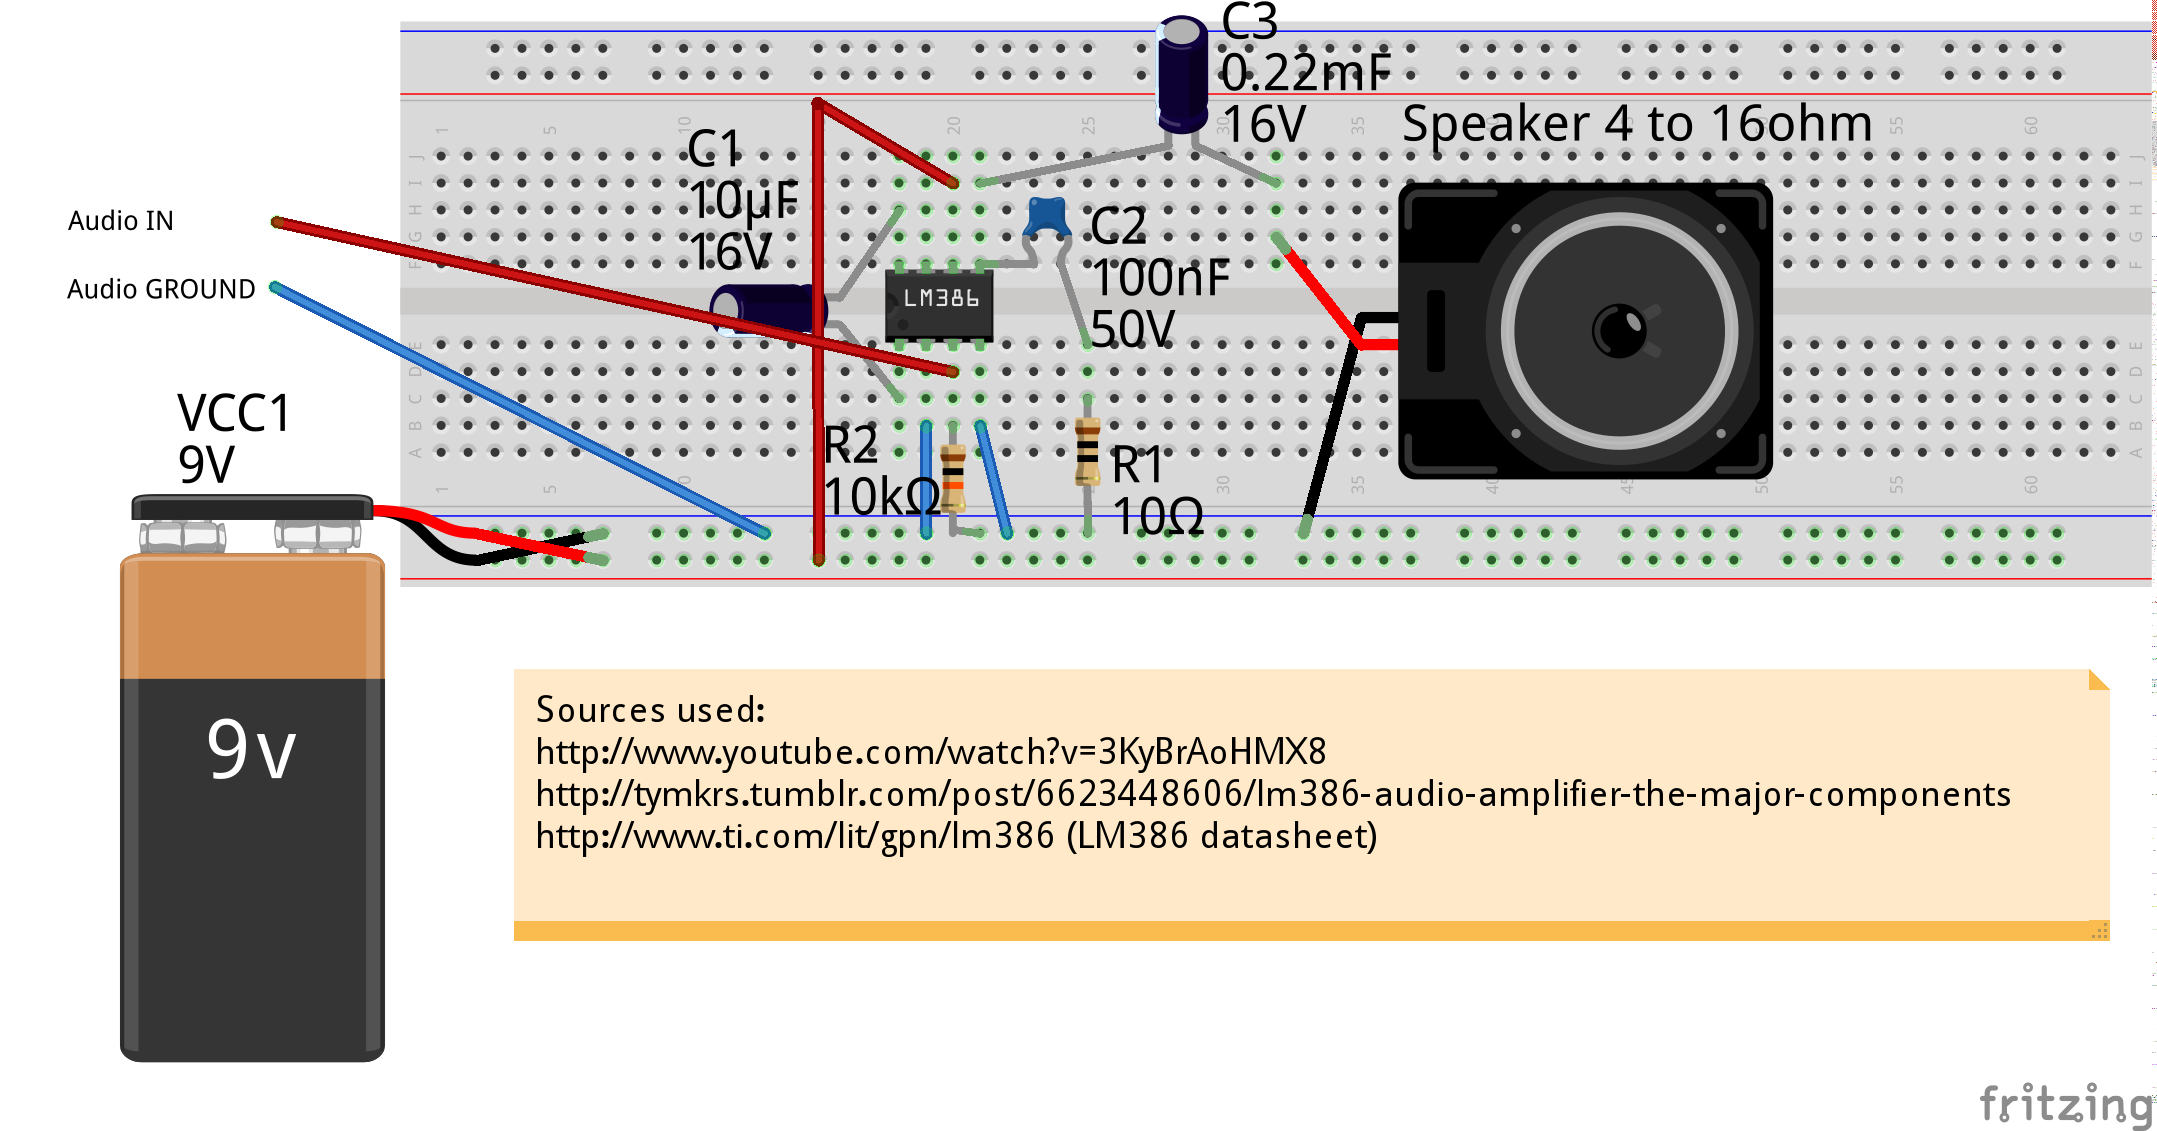
\includegraphics[scale=0.75]{audio_amplifier_lm386_bb.png}
    \caption{Breadboard view for the audio amplifier.}
  \end{center}
  \label{lm386_bb}
\end{figure}

In the heart of the audio amplifier stands the LM386 circuit, which is a "Low Voltage Audio Power Amplifier" and is more than enough for our use case. The figure in~\ref{lm386_bb} shows the breadboard view that we'll be using for the audio amplifier. The build is same to that what is shown on the LM386 datasheet, "amplifier with Gain = 200".

\begin{itemize}
  \item Between PINs 1 and 8 is a 10uF capacitor, which causes a gain on 200. In desibels this is around 20. 
  \item PIN 2 is places to ground.
  \item PIN 3 takes the audio input, and is connected to ground through 10k ohm resistor.
  \item PIN 4 is placed to ground.
  \item PIN 5 is the amplified audio output.
  \item PIN 6 takes power
  \item PIN 7 is bybassed, doesn't take connection.
\end{itemize}

\section{Camera}
Raspberry Pi Camera Board (https://www.element14.com/picamera) will be used for motion detection together with Raspberry Pi Userland code (https://github.com/raspberrypi/userland). At first, pictures will be taken using the raspistill-program provided by Userland. If we have time, we will integrate the camera code to be part of the other code, thus allowing us to strip all the unneeded features of userland.

Raspberry Pi has a camera socket intended for the camera, so no other electronic components are required in addition to the camera.

\section{Motors}
Lets assume that the turret has a weapon. In implementation the weapon will probably be either a laser pointer or an LED light. Moving the aim into correct position is done by two small DC motors, one for horizontal and one for vertical movement. Raspberry Pi will be controlling the motors via it's PCIO pins.

\begin{figure}
  \begin{center}
    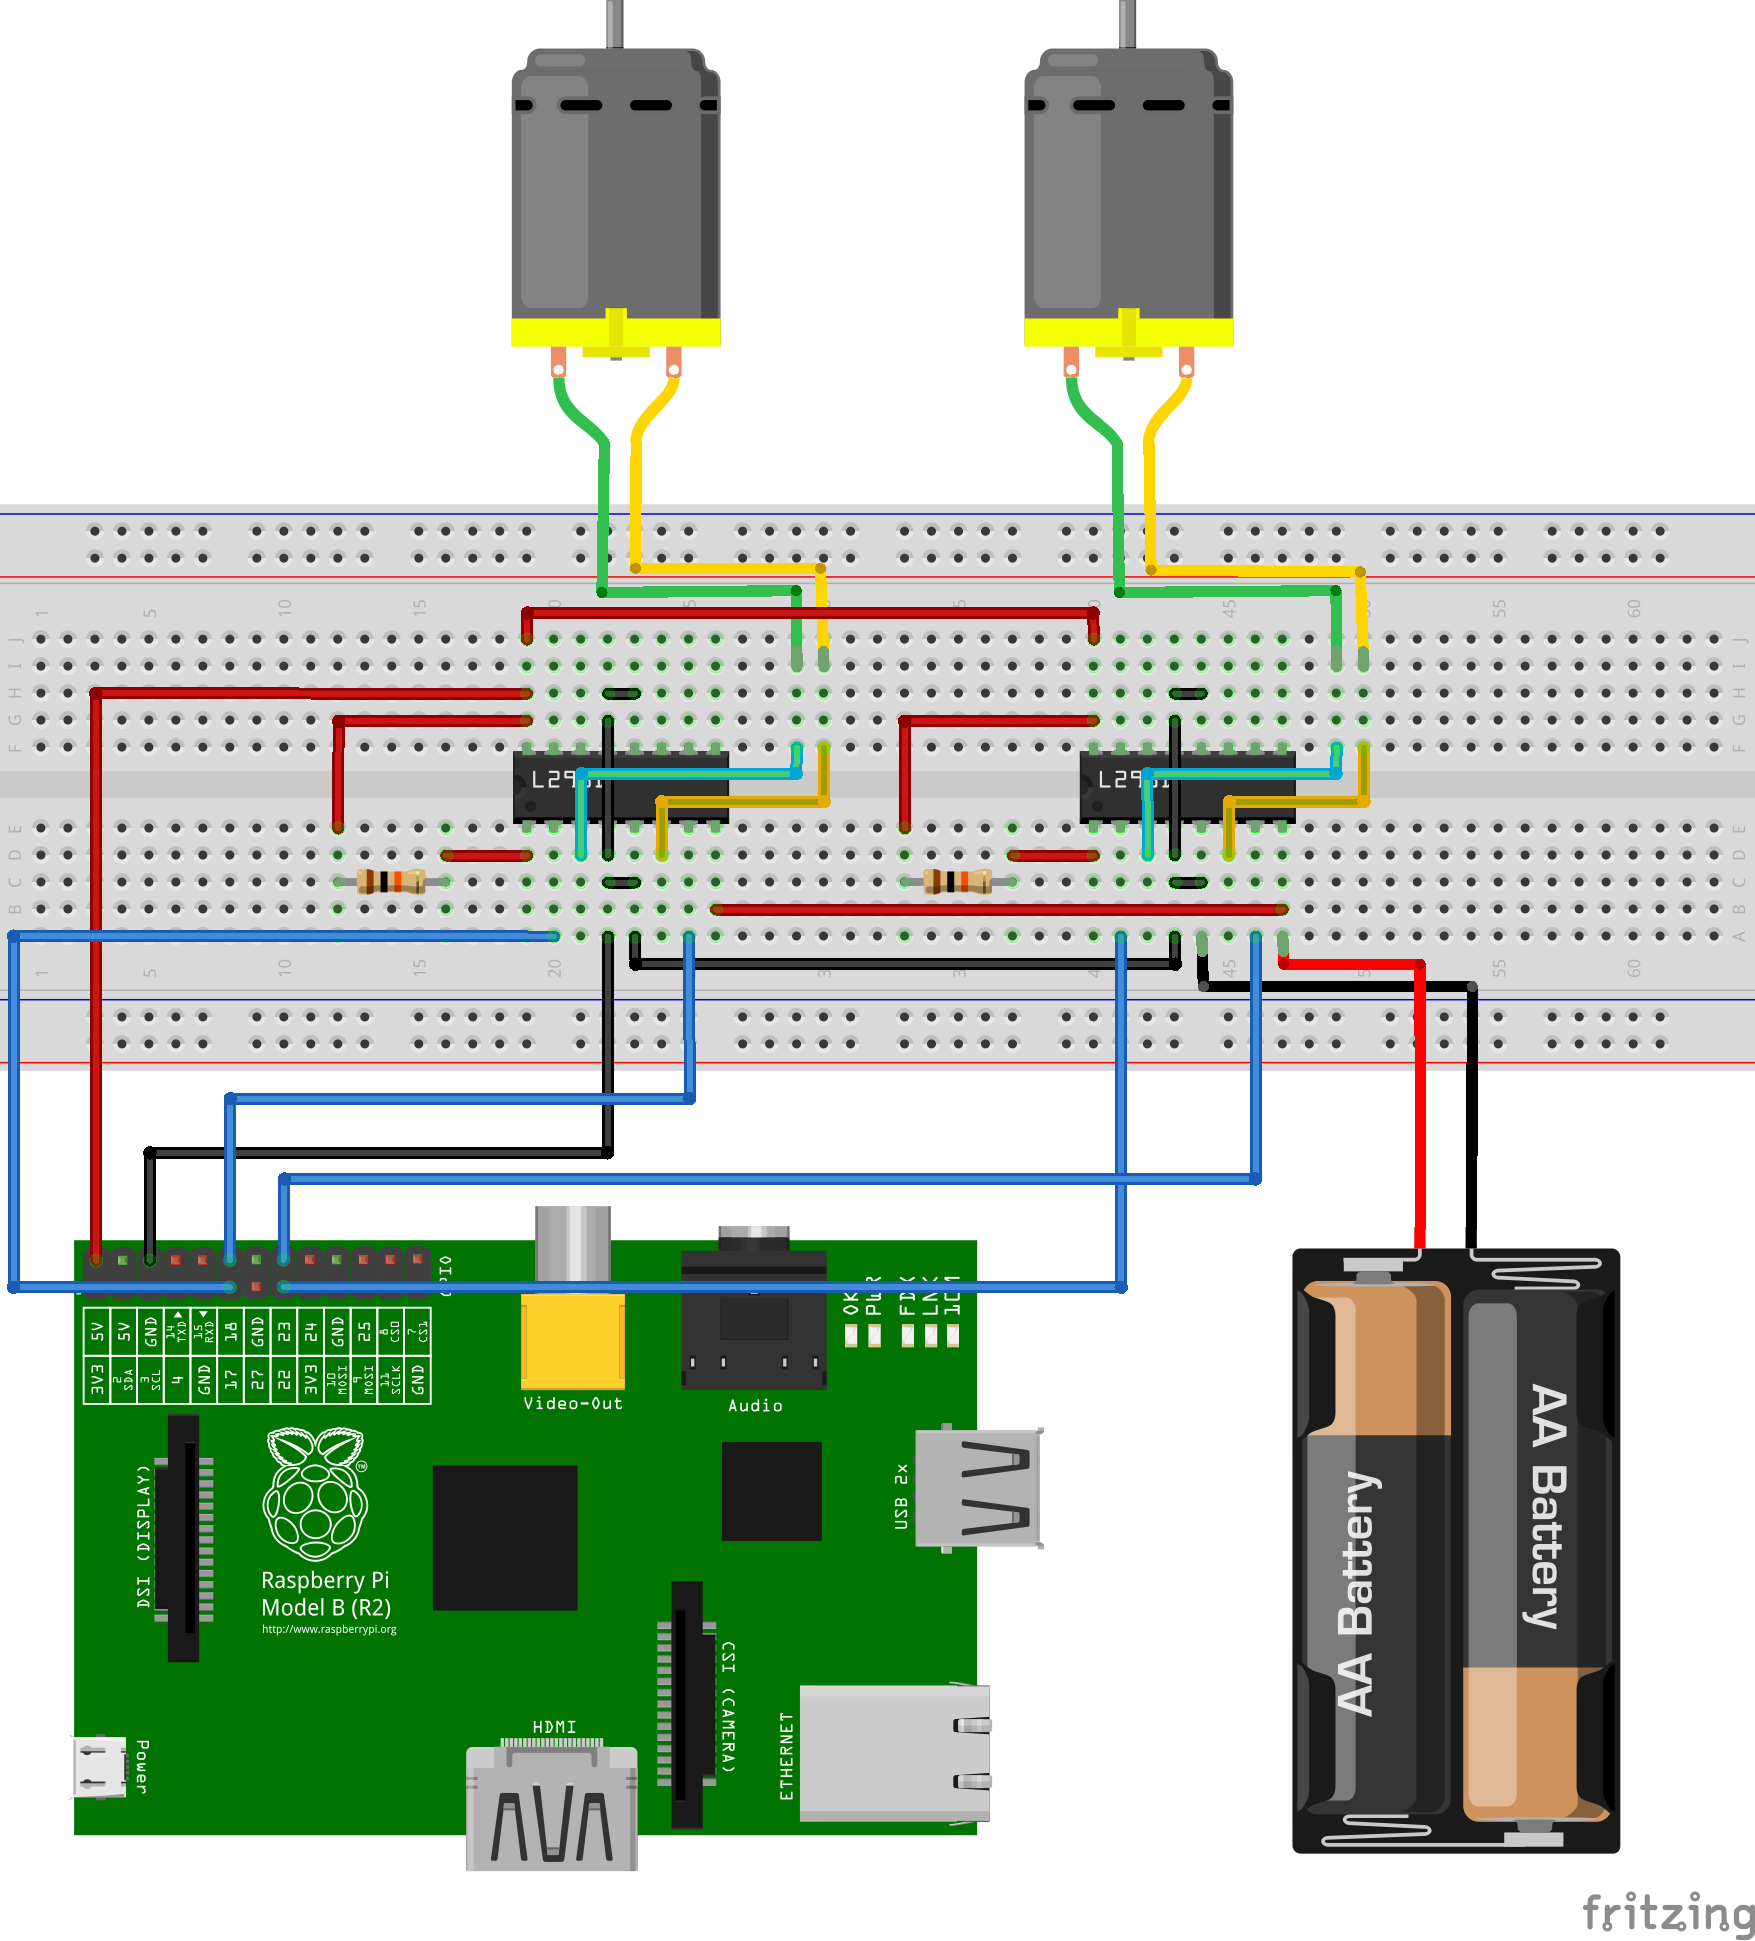
\includegraphics[scale=0.75]{motor_controllers_l293d_bb.png}
    \caption{Breadboard view for motor controllers.}
  \end{center}
  \label{l293d_bb}
\end{figure}

Our design uses two L293D motor controller chips for controlling the two motors. The breadboard design in figure \ref{l293d_bb} visualizes more closely on how the L293D chips are connected to Raspberry Pi, motors and additional battery power supply. The design shows how Raspberry Pi's GPIO pins 17 and 18 are used to control the first DC motor, and pins 22 and 23 are used to control the second one. L293D chips will get their VCC1 powers from the 5V Raspberry Pi pin, and their enable powers from the same pin, but trough 10 kilo ohm resistors. The motors will use power from two AA batteries, that give total of 3V voltage for the motors. Power for the motors are given through L293D chip's VCC2 pin.

A compact list for L293D chip's pin usage is the following:
\begin{itemize}
\item Pin 1: Enable signal for control signals \#1 and \#2.
\item Pin 2: Control signal \#1 input from Raspberry Pi.
\item Pin 3: Output current \#1 for the DC motor.
\item Pins 4-5: Ground 0V.
\item Pin 6: Control signal \#2 input from Raspberry Pi.
\item Pin 7: Output current \#2 for the DC motor.
\item Pin 8: VCC2 input, this is the motor's power current.
\item Pins 12-13: Ground 0V.
\item Pin 16: VCC1 power current for the 293D chip.
\end{itemize}

L293D motor control chip makes the DC motor turn left and right when control signals \#1 and \#2 from Raspberry Pi are in different states. If both of them are either low or high, the motor is stopped.

In order to test this design, we will code a simple testing software that gives correct signals from correct Raspberry Pi pins. After the software and signals are tested, then we will attach motor control chips into test bench to test how electronics work while connected. Only after these steps we can assemble our turret's mechanical parts.

\section{Software}
In addition to camera software provided by Raspberry Pi, we will write our own software for image analysis (motion detection), audio playback and motor movement. We will also write a remote control software for testing purposes at some point.

Our audio playback will be coded against pulseaudio sound server. The reason being, that it provides better API than ALSA. For example, there is \href{http://freedesktop.org/software/pulseaudio/doxygen/scache.html}{Sample cache} on the server side, which does sound optimal to what we're planning. We're planning to use ogg for audio files, but we'll see how it goes. We're not sure how much the Arm CPU of the Raspberry Pi can handle, adding ogg decoder on top of everything else might be too much. The first step is to just get somehow working nonblocking audio playback.

\end{document}
